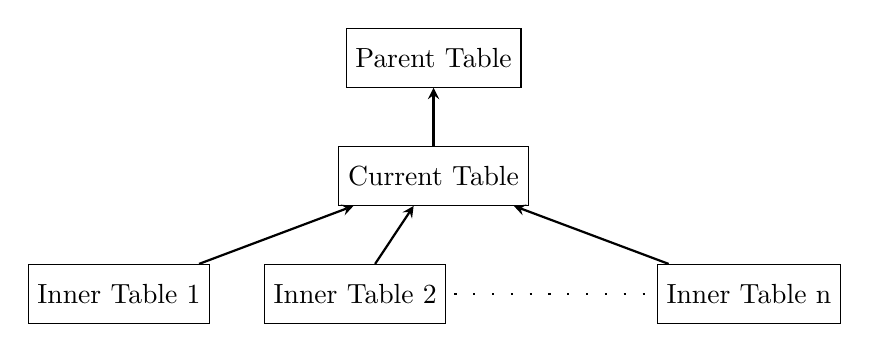
\begin{tikzpicture}[node distance = 3cm, 
                        symboltable/.style={draw, minimum height=0.75cm}]
        \node[symboltable](it1){Inner Table 1};
        \node[symboltable, right of=it1](it2){Inner Table 2};
        \node[symboltable, right of=it2, xshift=2cm](itn){Inner Table n};
        
        %\draw[ultra thick, loosely dotted] (it2) -- (itn);
        \path(it1)-- node[symboltable, yshift=1.5cm](ct){Current Table} (itn);
        \node[symboltable, yshift=1.5cm] (pt) at (ct) {Parent Table};
        
        \draw[stealth-, thick] (ct)edge(it1) edge(it2) edge(itn) edge[-stealth](pt);
        \draw[thick, dash pattern=on \pgflinewidth off 6pt, shorten >=0.1cm, shorten <=0.1cm] (it2)--(itn);
    \end{tikzpicture}